\documentclass{beamer}
% \usepackage{pgfpages}
% \pgfpagesuselayout{4 on 1}[a4paper,landscape,border shrink=5mm]
\usepackage{tikz}
\usetikzlibrary{shapes, backgrounds, arrows, positioning}
\usepackage{pgfplots}
\usepackage{listings}
\usepackage[utf8,latin1]{inputenc}
\usepackage[natbibapa]{apacite}
\makeatletter \def\newblock{\beamer@newblock} \makeatother  

\beamertemplatenavigationsymbolsempty
\setbeamertemplate{itemize items}[circle]
\setbeamertemplate{section in toc}[circle]
\mode<beamer>{\setbeamercolor{math text displayed}{fg=iwmgrau}}
\setbeamercolor{block body}{bg=iwmorange!50!white}
\setbeamercolor{block title}{fg=white, bg=iwmorange}

\definecolor{iwmorange}{RGB}{255,105,0}
\definecolor{iwmgrau}{RGB}{67,79,79}
\setbeamercolor{title}{fg=iwmorange}
\setbeamercolor{frametitle}{fg=iwmorange}
\setbeamercolor{structure}{fg=iwmorange}
\setbeamercolor{normal text}{fg=iwmgrau}
\setbeamercolor{author}{fg=iwmgrau}
\setbeamercolor{date}{fg=iwmgrau}
\color{white}

\title{Pre/post measurements}
\author{Nora Umbach%\footnote{These slides are a modified version of slides created by \url{https://osf.io/ /}. }
}
%\institute{\includegraphics[scale=.15]{figures/ut_logo}}
\date{May 17, 2021}
%\date{Last modified: \today}

\newcommand{\vect}[1]{\mathbf{#1}}
\newcommand{\mat}[1]{\mathbf{#1}}
\newcommand{\gvect}[1]{\boldsymbol{#1}}
\newcommand{\gmat}[1]{\boldsymbol{#1}}

\lstset{language=R,%
  literate={Ü}{{\"U}}1
           {ü}{{\"u}}1,
  %backgroundcolor=\color{iwmgrau!80!white},
  basicstyle=\ttfamily\color{iwmorange},
  frame=single,
  commentstyle=\slshape\color{black},
  keywordstyle=\bfseries\color{white},
  identifierstyle=\color{white},
  stringstyle=\color{green!85!black},
  numbers=none,%left,numberstyle=\tiny,
  basewidth={.5em, .4em},
  showstringspaces=false,
  emphstyle=\color{red!50!white}}

\lstdefinestyle{plain}{language=R,
  frame=none,
  basicstyle=\ttfamily\color{iwmorange},
  commentstyle=\slshape\color{iwmgrau},
  keywordstyle=\bfseries\color{iwmgrau},
  identifierstyle=\color{iwmgrau},
  stringstyle=\color{iwmgrau},
  numbers=none,
  basewidth={.5em, .4em},
  showstringspaces=false}

\pgfmathdeclarefunction{gauss}{2}{%
  \pgfmathparse{1/(#2*sqrt(2*pi))*exp(-((x-#1)^2)/(2*#2^2))}%
}

\AtBeginSection[]{
  \frame{
    \tableofcontents[sectionstyle=show/hide, subsectionstyle=show/show/hide]}}

\setbeamertemplate{headline}{
 \begin{beamercolorbox}{section in head}
   \vskip5pt\insertsectionnavigationhorizontal{\paperwidth}{}{}\vskip2pt
 \end{beamercolorbox}
}

\setbeamertemplate{footline}{\vskip-2pt\hfill\insertframenumber$\;$\vskip2pt}

\begin{document}

\begin{frame}{}
\thispagestyle{empty}
\titlepage
\end{frame}

\begin{frame}{Outline}
\tableofcontents
\end{frame}


\begin{frame}{Analyse von Longitudinaldaten}
Advantages

\begin{itemize}
\item More Power than cross sectional studies
\item Each subject is its own control person
\item Information of individual changes
\end{itemize}

Challenges
\begin{itemize}
\item Manche Testergebnisse nur ueber Simulationen verfuegbar
\item Fehlende Werte (Completer-Analyse, last observation carried forward,
  observed cases)
\item Praediktoren koennen sich ueber die Zeit veraendern
\item In Cross-Over-Designs: Carry-Over-Effekte
\end{itemize}
\end{frame}


\begin{frame}{Notation}
\begin{itemize}
\item $i = 1, \dots, N$ persons\\[2ex]

\item $j = 1, \dots, n_i$ time points for person $i$\\[2ex]

\item All observations: $\displaystyle\sum_i^N n_i$\\[2ex]

\item Vector of all observations for person $i$
\[
  (\vect{y}_i)_{n_i \times 1}
\]
%
\item Vector of covariates for person $i$ at time point $j$
\[
  (\vect{x}_{ij})_{p \times 1}
\]
%
\item All covariates of person $i$
\[
  (\vect{X}_i)_{n_i \times p}
\]
\end{itemize}
\end{frame}


\begin{frame}{Data schema}
\vfill
\begin{center}
\begin{tabular}{cccccc}
\hline
Person & Time      & Observation & \multicolumn{3}{c}{Covariates}\\\hline
1      & 1         & $y_{11}$    & $x_{111}$   & \dots & $x_{11p}$  \\
1      & 2         & $y_{12}$    & $x_{121}$   & \dots & $x_{12p}$  \\
.      & .         & .           & .           & \dots & .          \\
1      & $n_1$     & $y_{1n_1}$  & $x_{1n_11}$ & \dots & $x_{1n_1p}$\\
.      & .         & .           & .           & \dots & .          \\
.      & .         & .           & .           & \dots & .          \\
$N$    & 1         & $y_{N1}$    & $x_{N11}$   & \dots & $x_{N1p}$  \\
$N$    & 2         & $y_{N2}$    & $x_{N21}$   & \dots & $x_{N2p}$  \\
.      & .         & .           & .           & \dots & .          \\
$N$    & $n_N$     & $y_{Nn_N}$  & $x_{Nn_N1}$ & \dots & $x_{Nn_Np}$\\
\hline
\end{tabular}
\end{center}
\vfill
\end{frame}

\begin{frame}{$t$ test for dependent samples}
\begin{itemize}
  \item Most simple analysis for two measurements $n = 2$
  \item Written as linear model
    \begin{align*}
         d_i &= y_{i2} - y_{i1} \\
         d_i &= \beta_0 + \varepsilon_i \\
      y_{i2} &= \beta_0 + y_{i1} + \varepsilon_i
    \end{align*}
    with $\varepsilon_i \sim N(0, \sigma^2)$ i.i.d.
  \item Research question
  \begin{itemize}
    \item Is there change between the first and second time point ($H_0\colon \beta_0 = 0$)?
  \end{itemize}
  \item Which effects are not considered by this?
\end{itemize}
\end{frame}


\section{Zwei Messzeitpunkte}

\begin{frame}{Zwei Messzeitpunkte}
Design
\begin{itemize}
    \item Mindestens zwei Gruppen werden vor ($y_{i1}$) und nach ($y_{i2}$) einem Treatment beobachtet
        \begin{center}
        \begin{tikzpicture}
        \tikzstyle{every node}=[align=center]
        \node at (0.3, 3) (TG1) {TG1};
        \node at (0.3, 2.5) (TG2) {TG2};
        \node at (0.3, 2.1) (dots) {$\vdots$};
        \node at (0.3, 1.5) (CG) {CG};

        \node at (0, 1) (0) {};
        \node at (1.5, 1) [label=below:Baseline] (1) {};
        \node at (3, 1) (2) {$\cdots$};

        \node at (4.5, 1) [label=below:Treatment] (3) {};
        \node at (6, 1) (4) {$\cdots$};

        \node at (7.5, 1) [label=below:Follow-Up] (5) {};
        \node at (9, 1) (6) {};

        \foreach \x in {1.5, 4.5, 7.5} \draw[shift={(\x,1)}] (0pt,3pt) -- (0pt,-3pt);

        \draw               (0) -- (2);
        \draw               (2) -- (4);
        \draw[>=stealth,->] (4) -- (6) node[below] {$t$};
        \end{tikzpicture}
        \end{center}
    \item Fragestellung
    \begin{itemize}
      \item Unterscheiden sich die Gruppen in der Stärke der Veränderung?
    \end{itemize}
\end{itemize}
\end{frame}

\begin{frame}{t-Test zum Vergleich zweier Zeitpunkte}
\begin{itemize}
  \item Man betrachtet für jede Person den Change-Score $d_i = y_{i2} - y_{i1}$ und das Regressionsmodell
    {\color{iwmorange}\begin{align*}
         d_i &= \beta_0 + \varepsilon_i \\
      y_{i2} &= \beta_0 + y_{i1} + \varepsilon_i
    \end{align*}}
    mit $\varepsilon_i \sim N(0, \sigma^2)$ unabhängig
  \item Interpretation
    \begin{center}
    \begin{tabular}{ll}
    $\beta_0$ & mittlerer Change-Score
    \end{tabular}
    \end{center}
  \item Hypothese
    \begin{itemize}
        \item Gibt es eine Veränderung zwischen erstem und zweitem Zeitpunkt ($H_0\colon \beta_0 = 0$)?
    \end{itemize}
  \item Es bleibt unklar, ob die Veränderung auf das Treatment zurückzuführen oder Ergebnis eines Reifungsprozesses ist
\end{itemize}
\end{frame}


\begin{frame}{t-Test zum Vergleich zweier Zeitpunkte}
\begin{center}
\begin{tikzpicture}[>=stealth, y=.6cm, x=.6cm, font=\small]
\draw[->] (0,0) -- coordinate (x axis mid) (10,0);
\draw[->] (0,0) -- coordinate (y axis mid) (0,10);
\node[below=0.5cm] at (x axis mid) {Pre-treatment score, $y_1$};
\node[rotate=90, above=0.5cm] at (y axis mid) {Post-treatment score, $y_2$};
%
\draw (0, 1) -- (8, 9);
\draw (6, 7) -- (7, 7) -- (7, 7.5) node [right] {$1$} -- (7, 8);
\draw[dashed] (0, 6) node [above right] {$\beta_0$} -- (5, 6) -- (5, 0) node [below] {$0$};
\end{tikzpicture}
\end{center}
\end{frame}


\begin{frame}{t-Test der Follow-Up-Werte zweier Gruppen}
\begin{itemize}
  \item Regressionsdarstellung  mit $x_i = 1$, falls $i$-te Person zur Treatment-Gruppe gehört, und $0$ sonst:
    {\color{iwmorange}\[
      y_{i2} = \beta_0 + \beta_1 \, x_i + \varepsilon_i
    \]}
    mit $\varepsilon_i \sim N(0, \sigma^2)$ unabhängig
  \item Interpretation
    \begin{center}
    \begin{tabular}{ll}
    $\beta_0$ & mittlerer Follow-Up-Wert in Referenzgruppe\\
    $\beta_1$ & Effekt der Treatment-Gruppe
    \end{tabular}
    \end{center}
  \item Hypothese
    \begin{itemize}
        \item Unterscheiden sich die Gruppen zum zweitem Zeitpunkt ($H_0\colon \beta_1 = 0$)?
    \end{itemize}
  \item Da der Baseline-Wert unberücksichtigt bleibt, ist die Schätzung der Veränderung verzerrt
\end{itemize}
\end{frame}


\begin{frame}{t-Test der Follow-Up-Werte zweier Gruppen}
\begin{center}
\begin{tikzpicture}[>=stealth, y=.6cm, x=.6cm, font=\small]
\draw[->] (0,0) -- coordinate (x axis mid) (10,0);
\draw[->] (0,0) -- coordinate (y axis mid) (0,10);
\node[below=0.5cm] at (x axis mid) {Pre-treatment score, $y_1$};
\node[rotate=90, above=0.5cm] at (y axis mid) {Post-treatment score, $y_2$};
%
\draw (0, 5) node [above right] {$\beta_0 + \beta_1$} -- (9, 5) node [right] {TG};
\draw[dashed] (0, 3) node [above right] {$\beta_0$} -- (9, 3) node [right] {CG};
\end{tikzpicture}
\end{center}
\end{frame}

\begin{frame}{Change-Score-Analyse}
\begin{itemize}
  \item Regressionsdarstellung
    {\color{iwmorange}\begin{align*}
                  d_i &= \beta_0 + \beta_1 \, x_i + \varepsilon_i \\
      y_{i2} - y_{i1} &= \beta_0 + \beta_1 \, x_i + \varepsilon_i \\
               y_{i2} &= \beta_0 + y_{i1} + \beta_1 \, x_i + \varepsilon_i
    \end{align*}}
    mit $\varepsilon_i \sim N(0, \sigma^2)$ unabhängig
  \item Interpretation
    \begin{center}
    \begin{tabular}{lp{10cm}}
    $\beta_0$ & mittlerer Change-Score in  der Referenzgruppe\\
    $\beta_1$ & Differenz zu $\beta_0$ in der Treatment-Gruppe
    \end{tabular}
    \end{center}
  \item Hypothesen
    \begin{itemize}
        \item Gibt es eine Veränderung in der Referenzgruppe ($H_0\colon \beta_0 = 0$)?
        \item Unterscheidet sich die Veränderung in den Gruppen ($H_0\colon \beta_1 =0$)?
    \end{itemize}
\end{itemize}
\end{frame}


\begin{frame}{Change-Score-Analyse}
\begin{center}
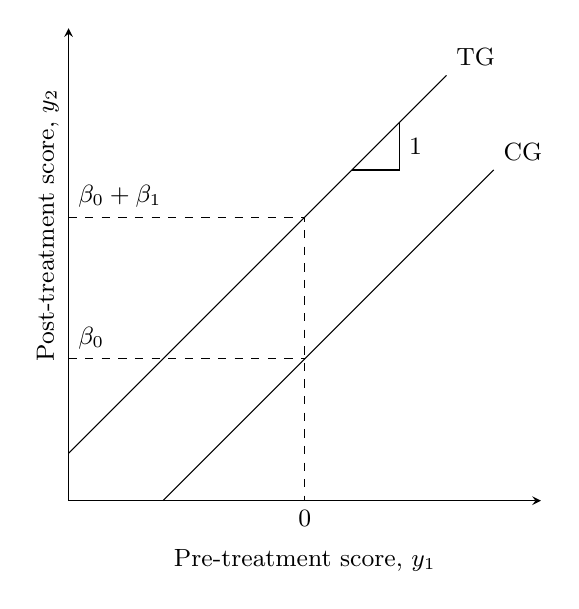
\begin{tikzpicture}[>=stealth, y=.6cm, x=.6cm, font=\small]
\draw[->] (0,0) -- coordinate (x axis mid) (10,0);
\draw[->] (0,0) -- coordinate (y axis mid) (0,10);
\node[below=0.5cm] at (x axis mid) {Pre-treatment score, $y_1$};
\node[rotate=90, above=0.5cm] at (y axis mid) {Post-treatment score, $y_2$};
%
\draw (0, 1) -- (8, 9) node [above right] {TG};
\draw (6, 7) -- (7, 7) -- (7, 7.5) node [right] {$1$} -- (7, 8);
\draw[dashed] (0, 6) node [above right] {$\beta_0 + \beta_1$} -- (5, 6) -- (5, 0) node [below] {$0$};
\draw (2, 0) -- (9, 7) node [above right] {CG};
\draw[dashed] (0, 3) node [above right] {$\beta_0$} -- (5, 3);
\end{tikzpicture}
\end{center}
\end{frame}



\begin{frame}{Regression zum Mittelwert}
\begin{itemize}
  \item Die Change-Score-Analyse basiert auf der häufig zu restriktiven Annahme, dass der Follow-Up-Wert vom Baseline-Wert mit Steigung $1$ abhängt
  \item Oftmals sind Baseline-Werte negativ mit den Change-Scores korreliert
    \begin{itemize}
      \item Personen mit niedrigen (schlechten) Werten verbessern sich stärker als Personen mit hohen Werten
    \end{itemize}
  \item Dieses als Regression zum Mittelwert bekannte Phänomen lässt also eine Steigung $< 1$ erwarten, die daher aus den Daten geschätzt werden sollte
\end{itemize}
\end{frame}

\begin{frame}{Kovarianzanalyse (ANCOVA)}
\begin{itemize}
  \item Regressionsdarstellung
    {\color{iwmorange}\[
      y_{i2} = \beta_0 + \beta_1 \, y_{i1} + \beta_2 \, x_i + \varepsilon_i
    \]}
    mit $\varepsilon_i \sim N(0, \sigma^2)$ unabhängig
  \item Interpretation
    \begin{center}
    \begin{tabular}{lp{10cm}}
    $\beta_0$ & mittlerer Follow-Up-Wert der Referenzgruppe für $y_{i1} = 0$\\
    $\beta_1$ & Effekt des Baseline-Werts\\
    $\beta_2$ & Differenz zum Follow-Up-Wert in der Treatment-Gruppe
    \end{tabular}
    \end{center}
  \item Hypothesen
    \begin{itemize}
        \item Hängen Baseline- und Follow-Up-Wert zusammen ($H_0\colon \beta_1 = 0$)?
        \item Unterscheiden sich die Follow-Up-Werte der Gruppen für Personen mit gleichem Baseline-Wert ($H_0\colon \beta_2 = 0$)?
    \end{itemize}
\end{itemize}
\end{frame}


\begin{frame}{Kovarianzanalyse (ANCOVA)}
\begin{center}
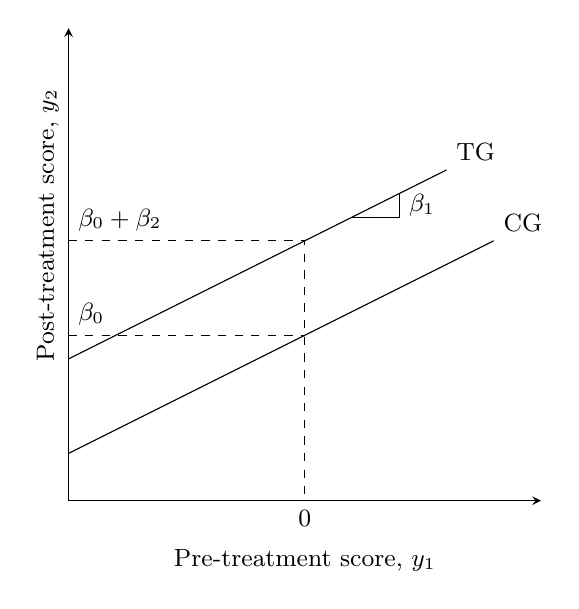
\begin{tikzpicture}[>=stealth, y=.6cm, x=.6cm, font=\small]
\draw[->] (0,0) -- coordinate (x axis mid) (10,0);
\draw[->] (0,0) -- coordinate (y axis mid) (0,10);
\node[below=0.5cm] at (x axis mid) {Pre-treatment score, $y_1$};
\node[rotate=90, above=0.5cm] at (y axis mid) {Post-treatment score, $y_2$};
%
\draw (0, 3) -- (8, 7) node [above right] {TG};
\draw (6, 6) -- (7, 6) -- (7, 6.25) node [right] {$\beta_1$} -- (7, 6.5);
%
\draw[dashed] (0, 5.5) node [above right] {$\beta_0 + \beta_2$} -- (5, 5.5) -- (5, 0) node [below] {$0$};
%
\draw (0, 1) -- (9, 5.5) node [above right] {CG};
\draw[dashed] (0, 3.5) node [above right] {$\beta_0$} -- (5, 3.5);
\end{tikzpicture}
\end{center}
\end{frame}


\begin{frame}{Adjustierte Mittelwerte}
\begin{itemize}
  \item Mit dem ANCOVA-Modell lassen sich für die Gruppen mittlere Follow-Up-Werte vorhersagen für Personen mit gleichem Baseline-Wert
  \begin{itemize}
      \item Beispielsweise erhält man
        \[
          \hat{y}_{i2} = \hat{\beta}_0 + \hat{\beta}_1 \, \bar{y}_1 +
                         \hat{\beta}_2 \, x_i
        \]
        für den durchschnittlichen Baseline-Wert $\bar{y}_1$
  \end{itemize}
  \item Diese bedingten Mittelwerte werden manchmal als (Baseline-)adjustierte Mittelwerte bezeichnet
\end{itemize}
\end{frame}


\begin{frame}{Unterschiedliche Steigungen in den Gruppen}
\begin{itemize}
  \item Regressionsmodell
    {\color{iwmorange}\[
      y_{i2} = \beta_0 + \beta_1 \, y_{i1} + \beta_2 \, x_i +
               \beta_3 \, (y_{i1} \cdot x_i) + \varepsilon_i
    \]}
    mit $\varepsilon_i \sim N(0, \sigma^2)$ unabhängig
  \item Interpretation
    \begin{center}
    \begin{tabular}{lp{10cm}}
    $\beta_0$ & mittlerer Follow-Up-Wert der Referenzgruppe für $y_{i1} = 0$\\
    $\beta_1$ & Effekt des Baseline-Werts\\
    $\beta_2$ & Differenz zum Follow-Up-Wert in der Treatment-Gruppe\\
    $\beta_3$ & Differenz zwischen Steigungen in Referenz-/Treatment-Gr.
    \end{tabular}
    \end{center}
  \item Hypothese
    \begin{itemize}
        \item Hängt der Effekt des Baseline-Werts von der Gruppe ab ($H_0\colon \beta_3 = 0$)?
    \end{itemize}
  \item Die Interpretation der adjustierten Mittelwerte unabhängig vom Baseline-Wert setzt $\beta_3 = 0$ voraus
\end{itemize}
\end{frame}


\begin{frame}{Interaktion zwischen Baseline-Wert und Gruppe}
\begin{center}
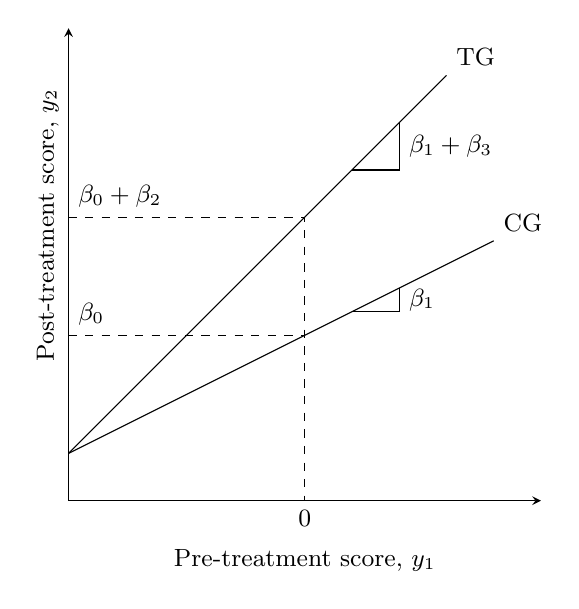
\begin{tikzpicture}[>=stealth, y=.6cm, x=.6cm, font=\small]
\draw[->] (0,0) -- coordinate (x axis mid) (10,0);
\draw[->] (0,0) -- coordinate (y axis mid) (0,10);
\node[below=0.5cm] at (x axis mid) {Pre-treatment score, $y_1$};
\node[rotate=90, above=0.5cm] at (y axis mid) {Post-treatment score, $y_2$};
%
\draw (0, 1) -- (8, 9) node [above right] {TG};
\draw (6, 7) -- (7, 7) -- (7, 7.5) node [right] {$\beta_1 + \beta_3$} -- (7, 8);
\draw[dashed] (0, 6) node [above right] {$\beta_0 + \beta_2$} -- (5, 6) -- (5, 0) node [below] {$0$};
%
\draw (0, 1) -- (9, 5.5) node [above right] {CG};
\draw (6, 4) -- (7, 4) -- (7, 4.25) node [right] {$\beta_1$} -- (7, 4.5);
\draw[dashed] (0, 3.5) node [above right] {$\beta_0$} -- (5, 3.5);
\end{tikzpicture}
\end{center}
\end{frame}


\begin{frame}{Kovarianzanalyse mit Change-Score}
\begin{itemize}
  \item Regressionsmodell
    {\color{iwmorange}\begin{align*}
                  d_i &= \beta_0 + \beta_1 \, y_{i1} + \beta_2 \, x_i + \varepsilon_i \\
      y_{i2} - y_{i1} &= \beta_0 + \beta_1 \, y_{i1} + \beta_2 \, x_i + \varepsilon_i \\
               y_{i2} &= \beta_0 + (1 + \beta_1) \, y_{i1} + \beta_2 \, x_i + \varepsilon_i
    \end{align*}}
  \item Für den Test des Unterschieds in der Veränderung in den Gruppen ($\beta_2$) spielt es keine Rolle, ob die Zielgröße der ANCOVA der Follow-Up-Wert oder der Change-Score ist
  \vfill
\end{itemize}
\end{frame}


\section{Beispiel: Akupunktur}


\begin{frame}{Beispiel}
Akupunktur bei Schulterschmerzen
\begin{itemize}
  \item Kleinhenz et al.\ (1999) untersuchten die Wirkung von Akupunktur auf die Verbesserung der Beweglichkeit bei 52 Patienten mit Schulterschmerzen
  \item Die Patienten wurden zufällig zwei Gruppen (Placebo und Akupunktur) zugewiesen
  \item Jeweils vor und am Ende der Behandlung wurde ein Beweglichkeitsscore erhoben
  \item Vickers und Altman (2001) zeigen am Beispiel dieser Daten die Vorteile der Kovarianzanalyse gegenüber anderen Verfahren
\end{itemize}
\end{frame}


\begin{frame}{Beispiel}
Akupunktur: Follow-Up-Analyse (Vickers \& Altman, 2001)
\begin{columns}[T]
\begin{column}{5.5cm}
  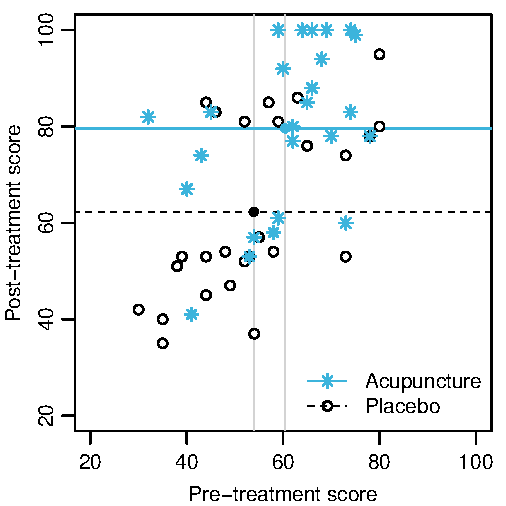
\includegraphics[width=5.5cm]{figures/acu-fwup}
\end{column}
%
\begin{column}{5.5cm}
  \vspace*{1em}\small
  \begin{tabular}{lrrr}
  \hline
             &  Pla &  Acu & Diff \\ \hline
  Baseline   & 53.9 & 60.4 &  6.5 \\
  Follow up  & 62.3 & 79.6 & 17.3 \\
  Change sc. &  8.4 & 19.2 & 10.8 \\
  ANCOVA     &      &      & 12.7 \\ \hline
  \end{tabular}
\begin{align*}
         y_{i2} &= \beta_0 + \beta_1 \, x_i + \varepsilon_i \\
  \hat{\beta}_1 &= 17.3, 0.95\text{ CI: } (7.5, 27.1)
\end{align*}
\end{column}
\end{columns}
\end{frame}


\begin{frame}{Beispiel}
Akupunktur: Change-Score-Analyse (Vickers \& Altman, 2001)
\begin{columns}[T]
\begin{column}{5.5cm}
  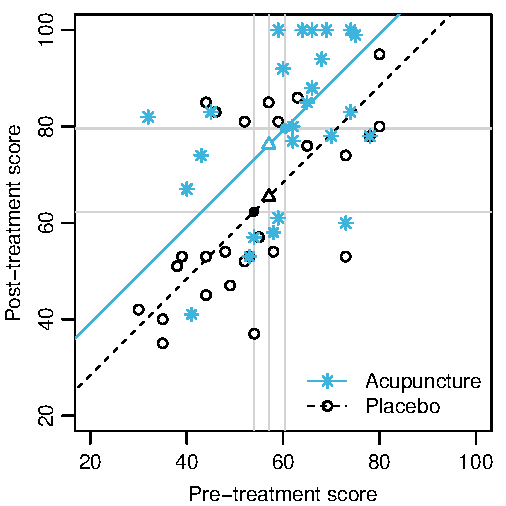
\includegraphics[width=5.5cm]{figures/acu-chng}
\end{column}
%
\begin{column}{5.5cm}
  \vspace*{1em}\small
  \begin{tabular}{lrrr}
  \hline
             &  Pla &  Acu & Diff \\ \hline
  Baseline   & 53.9 & 60.4 &  6.5 \\
  Follow up  & 62.3 & 79.6 & 17.3 \\
  Change sc. &  8.4 & 19.2 & 10.8 \\
  ANCOVA     &      &      & 12.7 \\ \hline
  \end{tabular}
\begin{align*}
         y_{i2} &= \beta_0 + y_{i1} + \beta_1 \, x_i + \varepsilon_i \\
  \hat{\beta}_1 &= 10.8 \; (2.3, 19.4)
\end{align*}
\end{column}
\end{columns}
\end{frame}


\begin{frame}{Beispiel}
Akupunktur: ANCOVA (Vickers \& Altman, 2001)
\begin{columns}[T]
\begin{column}{5.5cm}
  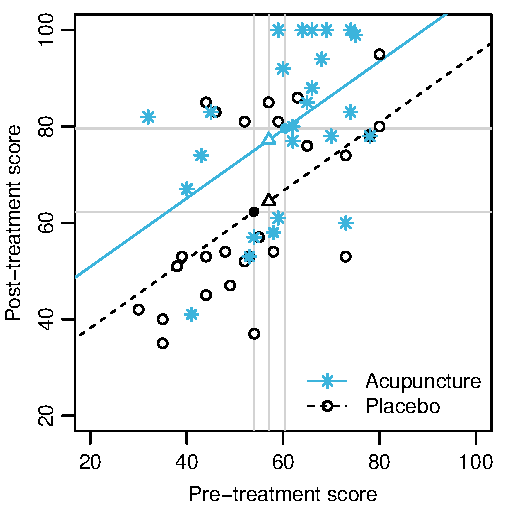
\includegraphics[width=5.5cm]{figures/acu-anco}
\end{column}
%
\begin{column}{5.5cm}
  \vspace*{1em}\small
  \begin{tabular}{lrrr}
  \hline
             &  Pla &  Acu & Diff \\ \hline
  Baseline   & 53.9 & 60.4 &  6.5 \\
  Follow up  & 62.3 & 79.6 & 17.3 \\
  Change sc. &  8.4 & 19.2 & 10.8 \\
  ANCOVA     &      &      & 12.7 \\ \hline
  \end{tabular}
\begin{align*}
         y_{i2} &= \beta_0 + \beta_1 \, y_{i1} + \beta_2 \, x_i +
                    \varepsilon_i \\
  \hat{\beta}_2 &= 12.7 \; (4.1, 21.3)
\end{align*}
\end{column}
\end{columns}
\end{frame}


\section{R-Demo}


\begin{frame}[fragile]{R-Demo}{}
%
Daten einlesen
\begin{lstlisting}
dat <- read.table("kleinhenz.txt", header=TRUE)
dat$grp <- factor(dat$grp, levels=c("plac", "acu"))
\end{lstlisting}
%\vspace*{-0.5em}

%
Follow-Up-Analyse
\begin{lstlisting}
m1 <- lm(post ~ grp, dat)
summary(m1)
confint(m1)
\end{lstlisting}
%\vspace*{-0.5em}

%
Change-Score-Analyse
\begin{lstlisting}
m2 <- lm(post ~ offset(pre) + grp, dat)
\end{lstlisting}
%\vspace*{-0.5em}

Kovarianzanalyse
\begin{lstlisting}
m3 <- lm(post ~ pre + grp, dat)
\end{lstlisting}
%\vspace*{-0.5em}
%
%
\end{frame}

\begin{frame}[fragile]{R-Demo}{}
%
Test auf gleiche Steigungen
\lstset{texcl=false}
\begin{lstlisting}
m4 <- lm(post ~ pre*grp, dat)
anova(m3, m4)
#   Res.Df   RSS Df Sum of Sq    F Pr(>F)
# 1     49 10998                         
# 2     48 10942  1     56.57 0.25   0.62
\end{lstlisting}
%\vspace*{-0.5em}

%
Adjustierte Mittelwerte
\lstset{texcl=false}
\begin{lstlisting}
predict(m3, data.frame(pre=mean(dat$pre),
        grp=c("plac", "acu")))
#    1    2 
# 64.5 77.2 
\end{lstlisting}
%\vspace*{-0.5em}
%
\end{frame}

\begin{frame}[fragile]{R-Demo}{}
%
Grafische Darstellung
\begin{lstlisting}
omean <- tapply(dat$post, dat$grp, mean)
pmean <- predict(m3, data.frame(pre=mean(dat$pre),
                 grp=c("plac", "acu")))
par(mai=c(.6, .6, .1, .1), mgp=c(2, .7, 0))
plot(post ~ pre, dat, type="n", xlim=c(20,100), ylim=c(20,100),
     xlab="Pre-treatment score", ylab="Post-treatment score")
abline(h=c(pmean, omean), v=c(mean(dat$pre),
                 tapply(dat$pre, dat$grp, mean)), col="lightgray")
xval <- 1:100
lines(predict(m3, data.frame(pre=xval, grp="plac")) ~ xval, lty=2)
lines(predict(m3, data.frame(pre=xval, grp="acu" )) ~ xval)
points(post ~ pre, dat[dat$grp == "plac", ], pch=21, bg="white")
points(post ~ pre, dat[dat$grp == "acu", ],  pch=8)
points(omean ~ tapply(pre, grp, mean), dat, pch=16)
points(pmean ~ rep(mean(pre), 2), dat, pch=24, bg="white")
legend("bottomright", c("Acupuncture", "Placebo"),
       pch=c(8, 1), lty=1:2, bty="n")
\end{lstlisting}
%\vspace*{-0.5em}
%
\end{frame}


\section{Zusammenfassung}


\begin{frame}{Zusammenfassung}
\begin{itemize}
  \item Die einfachste Art von Longitudinaldaten liegt vor, wenn mehrere Gruppen zu zwei Zeitpunkten beobachtet werden (Baseline und Follow-Up)
  \item Die Analyse solcher Daten bezieht sich dann auf die Differenzen
    \[
        d_i = y_{i2} - y_{i1}
    \]
    bzw.\ die adjustierten Follow-Up-Werte, die als unabhängig angesehen werden
  \item Die Kovarianzanalyse
  \begin{itemize}
    \item hat unter allen Verfahren die größte Teststärke, um Unterschiede in der mittleren Veränderung zu entdecken
    \item muss bei nicht-randomisierten Gruppen aber vorsichtig interpretiert werden
  \end{itemize}
\end{itemize}
\end{frame}


{\setbeamercolor{background canvas}{bg=iwmgrau!80!white}

\begin{frame}[fragile]{Poisson regression}
  \begin{lstlisting}
  ##\end{lstlisting}
\end{frame}

}

\begin{frame}[fragile]{}
  \begin{block}{Exercise}
    \begin{itemize}
      \item 
    \end{itemize}
  \end{block}
\end{frame}

% \appendix
% %\begin{frame}[allowframebreaks]{References}
% \begin{frame}{References}
% \renewcommand{\bibfont}{\footnotesize}
% \bibliographystyle{apacite}
% \bibliography{../../../literature/nu}
% \vfill
% \end{frame}

\end{document}

